% !Mode:: "TeX:UTF-8" 

\BiChapter{跨项目克隆代码一致性维护需求预测实证研究}
{An Empirical Study on Clone Consistency Prediction for Cross-Project}


\BiSection{引言}
{Introduction}

%由于日益增长的软件开发的需求,开发人员在软件开发过程中通过复制粘贴既有代码,向系统中引入了大量克隆代码。
克隆代码的变化包含克隆代码创建和修改,在克隆代码的演化过程中会引起一致性变化的问题。本文在第三章和第四章分别在克隆代码创建时和变化时,对克隆代码的一致性维护需求进行了预测。但是,上述方法可以适用于经过若干版本演化后具备充分的数据的实验系统上。对于时间较短的软件系统,由于未经过充分演化,系统中可能无法收集到充分的数据,进而无法较好的训练机器学习模型。因此,本章借鉴软件缺陷预测领域中的跨项目预测方法,在第三章和第四章研究的基础上,对跨项目的克隆代码一致性维护需求预测问题进行实证研究。跨项目的克隆代码的一致性预测研究,可以在软件开发初期帮助程序开发人员避免克隆代码导致的额外维护代价和克隆一致性缺陷,从而帮助提高软件质量和可维护性。

\textcolor{red}{本章对跨项目的克隆代码的一致性预测问题进行了实证研究,使用其它项目的数据训练模型并预测另外项目的一致性预测问题。本章首先提出了本章的研究问题,并统一了克隆代码的一致性变化维护需求定义,对克隆代码的一致性维护需求预测进行跨项目的实证研究。针对所提出的问题首先通过构建软件系统的克隆家系来收集系统中所有的克隆实例(克隆创建实例和克隆变化实例),并提取不同的属性值表示不同的克隆实例。然后,使用五种不同的机器学习方法,分别在克隆创建时和变化时预测克隆代码的一致性维护需求。最后,结合软件开发过程,设计并实现了克隆代码一致性维护需求预测插件(CCRP),并可以嵌入到集成开发环境eclipse中预测克隆代码一致性需求。本章在四个开源软件系统上进行了实证研究,实验结果表明本文所提取的属性值可以适用于不同的机器学习方法上,且支持向量机方法更适合于克隆代码的一致性维护需求预测中。本章基于eclipse所实现的插件,可以帮助开发人员在软件开发过程中预测克隆代码的一致性,降低克隆代码导致的额外的维护代价,避免克隆变化导致的一致性缺陷,从而提高软件质量和可维护性。}


\BiSection{跨项目克隆代码一致性维护需求}
{Clone Consistency-Requirement}

\BiSubsection{研究问题}
{Research Problem}

在软件开发过程中,通过复制粘贴操作复用既有代码已经成为一种常见的软件开发手段,但是也会向软件系统中引入大量的克隆代码。这些新创建的克隆代码以及系统已经存在的克隆代码并不是静止不变的,会随着软件系统演化。在演化过程中,克隆片段片段可能会被软件开发员修改而发生变化,并可能进一步引发克隆组的一致性变化。克隆代码的一致性变化问题会影响软件质量和可维护性,原因在于:程序开发人员需要对发生变化的克隆进行一致性维护,会导致额外的一致性维护代价。而遗忘克隆的一致性变化,更会会导致克隆不一致缺陷,从而进一步增加软件的维护代价。

为了解决此问题,本文的第三章和第四章分别在克隆代码创建时和变化时对克隆代码的一致性维护需求进行了预测,并取得了不错的预测效果。但是,上述方法中仅仅仅仅考虑了系统中具有充分的数据对机器学习模型进行训练,未考虑训练数据不足的情况。即在软件开发的初始阶段,由于软件系统刚刚开始演化,系统中并没有充足的克隆创建实例和克隆变化实例,因此,使用这些不充足的训练数据会导致模型训练不够完全,从而无法在软件开发的初始阶段对其进行克隆代码的一致性维护需求预测问题。因此,这启发了本章对跨项目的克隆代码的一致性维护需求的研究。

为了更好地帮助软件开发人员维护克隆代码,并解决软件开发初期训练数据不足的问题,本章将参考缺陷预测中跨项目预测的方法,对克隆代码的一致性维护需求进行跨项目的预测研究。具体地,本章地研究问题如下:

\textbf{Research Problem: 能否使用跨项目的数据,去预测克隆代码的一致性维护需求预测,且软件开发人员应如何结合软件开发过程中执行克隆一致性需求预测?}\\

为了解决本章的研究问题,将从不同的角度研究跨项目的克隆代码的一致性维护需求预测问题。在预测克隆一致性的过程中充分考虑并结合软件开发过程,从而帮助开发人员实际开发环境中执行克隆代码一致性预测,具体地,本文章研究问题可以细分为以下三个子问题,如下所示:

%%{\bf RQ1:}
%%能否使用跨项目的数据
%%
%%{\bf RQ2:}
%%在预测克隆代码变化时的一致性维护需求时,哪些机器学习方法可以用于该预测中,且所提取得度量值能否应用于其他的机器学习方法中,不同的机器学习方法预测效果是否一致,哪一种机器学习的方法能够取得最好的结果?
%%
%%
%%{\bf RQ3:}
%%在实际开发过程中,程序开发人员应该如何结合软件开发过程选择合适的机器学习模型和预测时间,并对克隆代码进行一致性维护需求进行预测,从而都够达到最佳的预测效果?


\BiSubsection{克隆一致性维护需求定义}
{The Definitions for Clone Consistency-Requirement}

在克隆代码的整个演化周期中,克隆片段可能会被开发人员修改,从而导致克隆代码的一致性变化。在本文的第三章和第四章分别提供了两种不同形式的克隆代码一致性变化定义,从而适应于不同时间的克隆一致性维护需求预测中。为了进一步研究跨项目的一致性预测问题,本章统一了第三章和第四章的定义,以应用于本章的实证研究中。具体来说,克隆代码的一致性变化如下:\\

\begin{definition}
[一致性变化]  
\label{def-change}
给定两个克隆代码片段 $CF_1$和 $CF_2$,且它们被分别地修改为$CF'_1$和$CF'_2$。 如果对于一个非常小的阈值$\tau$,如果克隆代码$CF_1$和$CF_2$的变化满足以下条件,称此变化为一致性变化(Consistent Change) , 
  \[
  \begin{array}[t]{crl}
    \mathit{textSim}(CF_i, CF'_i) < 1 & \forall i \in \{1,2\} &(1) \\
    \multicolumn{2}{c}{| ~\mathit{textSim}(CF_1,CF'_1)  ~-~ \mathit{textSim}(CF_2,CF'_2) ~| ~< ~ \tau}  & (2)
  \end{array}
  \]
更具体地,如果克隆变化仅满足条件1,将其称为Type-1一致性变化({\em Type-1 Consistent Change});如果克隆变化同时满足条件1和条件2,将其称为Type-1一致性变化({\em Type-2 Consistent Change})。
\end{definition}

%\begin{definition}[{\bf Consistent Change}]  
%\label{}
%Given that two clone fragments $CF_1$, $CF_2$ are modified to $CF'_1$ and $CF'_2$ respectively. 
%We say this modification on $CF_1$ and $CF_2$ is a {\em\bf consistent change\/} if for some very small threshold $\tau$, 
%  \[
%  \begin{array}[t]{crl}
%    \mathit{textSim}(CF_i, CF'_i) < 1 & \forall i \in \{1,2\} &(1) \\
%    \multicolumn{2}{c}{| ~\mathit{textSim}(CF_1,CF'_1)  ~-~ \mathit{textSim}(CF_2,CF'_2) ~| ~< ~ \tau}  & (2)
 % \end{array}
 % \]
%More specifically, if they only satisfy condition 1, we call this as {\bf \em type-1 consistent change}, and if both conditions 1 and 2 are satisfied, we term it {\bf \em type-2 consistent change}.
%\end{definition}

定义中克隆代码$ CF_1 $和$ CF_2 $的变化情况由相似性度量$ \mathit {textSim} $进行定义,$textSim$与第三章和第四章计算方式相同。定义中的两个约束条件共同定义了克隆代码的一致性变化,约束条件$1$确保了克隆代码片段同时被修改,约束条件$2$克隆代码片段发生了一致性的变化,由变化阈值$\tau$指定。

其中,Type-1一致性变化又可以称为克隆创建时一致性变化,Type-2一致性变化又称为克隆变化时的一致性变化。这两种不同的一致性变化,将分别应用于两种不同时间的克隆一致性预测中。在克隆代码创建时,目标是避免新创建的克隆代码在其未来演化过程中的一致性变化,及其所导致额外的维护代价。所以,只要两个克隆片段同时变化,即认为会导致额外维护代价。因此,在克隆代码创建时使用使用Type-1一致性变化进行预测。在克隆代码变化时,目的是避免克隆变化可能导致的未来演化中的一致性变化,及其因此所引发的克隆一致性缺陷。所以, 不仅要求两个克隆代码片段同时变化,还需要发生相似的变化,否则将会引入克隆一致性缺陷,因此,在克隆代码变化时使用使用Type-2一致性变化进行预测。

在克隆演化过程中,克隆片段是以克隆组的形式出现在软件系统中。克隆代码的变化情况必然会导致克隆组的变化,而克隆组的变化使用克隆演化模式进行描述,即一致性变化模式。本文给出演化过程中克隆组的一致性变化模式定义,如下所示:\\


\begin{definition}
[一致性变化模式] 
\label{def-pattern}
在软件版本 $j+1$中存在一个克隆组$CG'$ ,假设克隆组内至少存在两个克隆代码片段$CF'_1$ 和 $CF'_2$可以与映射到上一版本$j$的克隆组$CG$中,且 $CG$中与之对应的克隆代码片段的 $(CF_1,CF_2)$被修改为$(CF'_1,CF'_2)$。如果克隆片段之间的变化( $(CF_1,CF_2)$变化至$(CF'_1,CF'_2)$满足克隆片段的“一致性变化(Consistent Change)”,则称克隆组$CG'$具有一致性变化模式(Consistent Change Pattern)。
\end{definition}

%\begin{definition}[{\bf Consistent Change Pattern}] 
%\label{}
%{\em
%A clone group $CG'$ in software version $j+1$ possesses {\em\bf type-1 or 2 consistent change pattern} if there exists a pair of clones $CF'_1,$ and $CF'_2$  in $CG'$ which are mappable to a pair of clones $CF_1$ and $CF_2$ in a clone group $CG$ in version $j$ such that modification of code pairs from $(CF_1,CF_2)$ to $(CF'_1,CF'_2)$ is a type-1 or 2 consistent change. 
%} 
%\end{definition}

其中“一致性变化”为Type-1或Type-2一致性变化,相应的克隆组变化模式则为Type-1和Type-2一致性变化模式。在相邻的两个软件版本中,克隆组一致性变化模式可以描述克隆演化中由于克隆片段变化所引发的克隆组的变化情况。

回顾本章地研究内容是要在两种不同的时刻预测克隆代码的一致性维护需求,结合第三章和第四章的克隆实例的定义,这里将统克隆创建实例和克隆变化实例为克隆代码实例,如下所示:\\

\begin{definition}
[克隆实例] 
\label{def-instance}
克隆创建实例:软件版本 $j$中的一个克隆组$CG$是克隆创建实例,如果该克隆组$CG$是其克隆家系$CGE$的根节点。
克隆变化实例:
软件版本 $j$中的一个克隆组$CG$是克隆变化实例,如果克隆组$CG$中至少两个克隆片段发生变化且版本$j+1$ 中至少存在一个克隆组$CG'$与之对应(在同一克隆家系$CGE$中)。 
克隆实例: 将克隆创建实例和克隆变化实例统称为克隆实例。
\end{definition}
%In the above definitions, we identify a $CG$ created by a creating operation (copy and paste) as a new $CGE$ root that begins its evolution. 

%\begin{definition}[{\bf Clone Instance}] 
%\label{}
%{\bf Clone Creating Instance:}
%{\em 
%A clone group $CG$ in version $j$ is {\bf clone creating instance} if $CG$ is a root node in the clone genealogy ($CGE$). 
%}
%~\\
%{\bf Clone Changing Instance:}
%{\em A clone group $CG$ in version $j$ is a {\bf clone changing instance} if at least one clone group $CG'$ in version $j+1$ which is connected to $CG$ in the clone genealogy was modified. 
%}
%~\\
%{\bf Clone Instance:}
%{\em We call clone creating and changing instance as {\bf clone instance}.
%}
%\end{definition}


克隆实例在演化过程中可能会引发的克隆一致性变化,如果不能确保克隆的一致性,将会导致导致额外的维护代价和一致性缺陷。具体来说,对于克隆创建实例,本文认为Type-1一致性变化及其演化模式在克隆演化过程中可能会导致额外的克隆维护代价。对于克隆变化实例,本文认为Type-2一致性变化及其演化模式在克隆演化过程可能会导致克隆一致性缺陷。因此,本章尝试在不同的时间预测克隆实例的一致性维护需求,以避免额外的克隆维护代价和一致性缺陷。本章结合第三章和第四章的克隆代码一致性维护需求的定义,将克隆创建时和变化时的一致性维护需求统一为克隆一致性维护需求定义,如下所示:\\

\begin{definition}
[克隆一致性维护需求] 
 \label{def-requirement}
给定版本 $j$中一个克隆实例,$CG$满足克隆一致性维护需求(Consistency-Requirement),如果在版本$k$中存在一个克隆实例 $CG'$($k>j$)满足以下条件: (1) 在$CG'$中至少存在两个克隆片段在其克隆家系$CGE$中可以映射到克隆实例 $CG$中, (2) $CG'$ 具有“一致性变化模式”(Consistent Change Pattern)。反之,假如克隆实例$CG$ 不满足克隆一致性维护需求条件,称该克隆实例不需要一致性维护(consistency-requirement free,或者consistency-free)。
\end{definition}

%\begin{definition}[{\bf Clone Consistency-Requirement}] 
 %\label{}
%{\em
%A clone instance $CG$ in software version $j$ satisfies {\bf consistency-requirement\/} condition if there is a clone group $CG'$ in software version $k$, with $k>j$, such that (1) there is at least a pair of clones in $CG'$ that is mappable in clone genealogy to a pair of clones in $CG$, and (2) $CG'$ possesses ``consistent change pattern''. When $CG$ does not satisfy consistency-requirement, we say that it is {\bf consistency-requirement free\/}, or simply {\em consistency-free\/} or {\em free} for short. %\\
%We employed the type-1 consistent change pattern for clone creating instance, and type-2 for changing instance.c
%}
%\end{definition}

其中,“一致性变化模式”为Type-1或Type-2一致性变化模式,相应的克隆一致性需求为Type-1和Type-2一致性维护需求。其中,Type-1克隆一致性维护需求可以用于预测克隆创建实例,Type-1克隆一致性维护需求可以用于预测克隆变化实例。

最终,克隆一致性维护需求预测任务可以转化为以下问题:
%{\bf Prediction Task:}
 给定一个克隆实例,克隆创建实例或者克隆变化实例,判断该克隆实例是否满足克隆一致性维护需求。
 
 更进一步,本文将克隆代码一致性维护需求预测问题转换成为一个分类问题,因而可以使用机器学习中的方法来解决此问题。在本文第三章和第四章的研究中,仅仅考虑了贝叶斯网络方法,为了更深入研究克隆代码的一致性预测问题,本文将会使用五种不同的机器学习方法在预测克隆实例的一致性维护需求。将在后文中详细介绍。


\BiSection{ 跨项目的克隆代码一致性需求预测框架}
{The Framework for Clone Consistency-Requirement of Cross-Project}

为解决本章所提出的跨项目的克隆代码一致性需求维护预测问题,本文首先给出了一个方法框架。跨项目的克隆代码一致性需求预测框架如图~\ref{framework5}~所示。跨项目的克隆代码方法可以划分为三个阶段,分别为训练数据收集阶段、测试数据收集阶段和跨项目预测阶段。收集阶段旨在收集训练系统和测试系统中全部的克隆实例(包括创建实例和变化实例),并将训练系统的数据集用于机器学习模型的构建,测试系统的数据用于测试跨项目预测的效果。在预测阶段,使用训练系统所构建的机器学习模型预测测试系统的克隆代码一致性维护需求。%值得注意的是,将分别由于实际的克隆实例无法直接应用于机器学习方法中,因此在表示步骤中将提取不同的属性值表示克隆实例,所提取的属性值将包含克隆实例的有意义的信息。接下来,在预测步骤,使用属性化的克隆实例构建和训练机器学习模型,并使用其预测克隆实例的克隆一致性维护需求。


\begin{figure}[htbp]
\centering
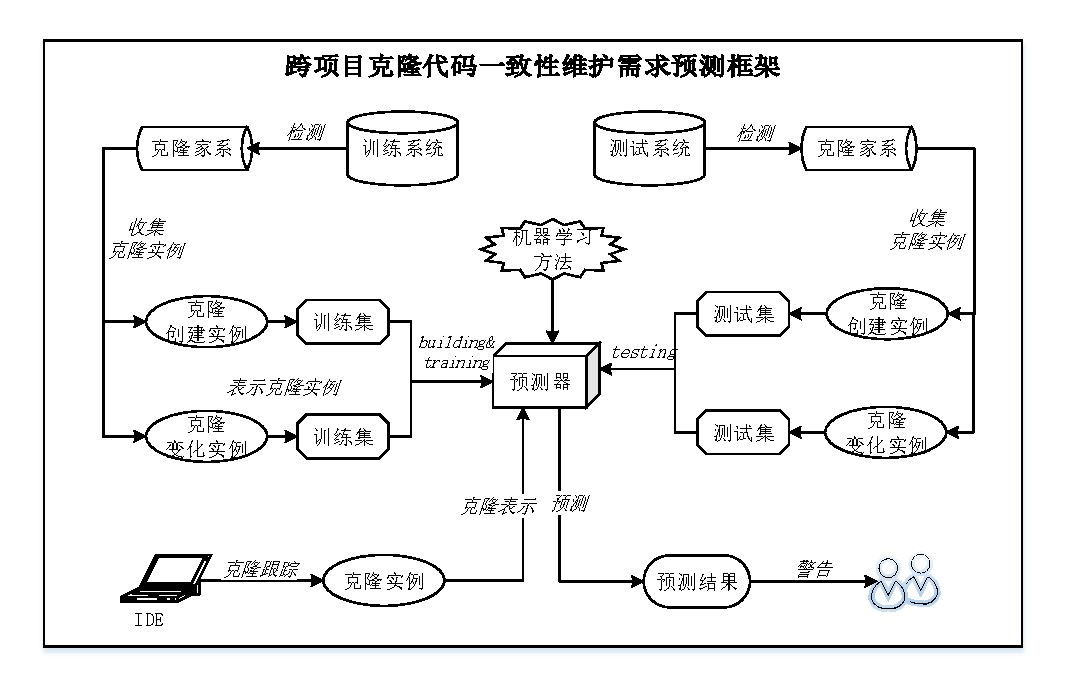
\includegraphics[width = 0.9\textwidth]{framework5.pdf}
\bicaption[framework5]{}{跨项目克隆代码一致性维护需求预测框架}
{Fig.$\!$}{The framework for clone consistency prediction of cross-project}
\vspace{-1em}
\end{figure}

具体来说,在收集阶段中,通过构建系统的克隆家系从相关软件系统中收集所有的克隆实例。使用NiCad来检测软件版本中的所有克隆,并通过在相邻版本的克隆组之间进行映射来构建克隆家系,用于识别克隆实例。然后,通过提取属性值表示克隆创建和变化实例,提取代码属性和上下文属性表示克隆创建实例,提取代码属性、上下文属性和历史属性表示克隆变化实例。在预测阶段中,使用收集到的训练系统的克隆实例训练机器学习模型,并使用其预测测试系统的克隆代码一致性维护需求。

%克隆实例有两种不同的预测结果,即满足一致性维护需求和不满足维护需求。
对于满足一致性维护需求实例来说,其在将来的演化中可能会引发一致性变化,程序开发人员需要采取相应的操作。例如,拒绝克隆创建实例或者检查克隆变化实例一致性。对于不满足一致性维护需求实例来说,其在将来的演化中不会引发一致性变化,程序开发人员需要采取相应的操作,如接受克隆创建实例。

%本章使用多个不同的机器学习模型预测克隆实例的一致性。所提取的克隆实例的属性即为机器学习模型中的输入特征,用于构建不同机器模型的结构。所收集到的克隆变化实例可作为机器学习的训练集,用于训练机器学习模型的相关参数,细节可参考本文后续章节。本章使用和比较五种不同的机器学习方法,以帮助开发人员选择最佳的预测手段。
同时,测试系统和训练系统数据收集方法与过程,与第三章和第四章中的方法相似,通过收集和表示系统中的克隆实例完成。

\BiSection{克隆实例收集和表示}
{Collecting and Representing Clone Instance}

收集和表示克隆实例可以生成克隆一致性预测的训练集,为将克隆实例应用于机器学习中,提取不同的属性值表示克隆实例,从而可以训练机器学习模型。

\BiSubsection{克隆实例收集}
{Collecting Clone Instances}

收集克隆实例的目的在于生成克隆一致性预测的训练集,并将其用于训练机器学习模型。通过构建系统的克隆家系并识别其中的克隆演化模式,可以从软件中收集所有的克隆实例。首先使用NiCad来检测软件版本中的所有克隆,然后通过在相邻版本的克隆组之间进行映射来构建克隆家系,最后识别Type-1和Type-1克隆一致性演化模式识别系统中的克隆创建和变化实例。

根据定义~\ref{def-instance}~,克隆家系$CGE$中的初始节点即是克隆创建实例,发生变化的克隆组是变化实例,因此因此通过构建克隆家系可以收集克隆创建和变化实例。

(1)构建克隆家系。首先,下载系统所有版本的源代码,并使用NiCad的默认配置检测检测每一版本的中Type1-3的克隆代码。然后,通过映射所有相邻版本的克隆代码,构建系统中全部克隆家系。为完成版本间的映射,为每个克隆片段生成一个克隆区域描述符 $CRD$\cite{duala2010clone},使用基于$CRD$的克隆映射算法映射两个连续版本之间的所有克隆片段和克隆组\cite{ci2013new}\cite{ci2013newD}。根据克隆映射结果,构建系统的克隆家系。

(2)识别克隆演化模式和收集克隆实例。首先,识别克隆家系中的克隆演化模式,尤其是克隆一致性变化模式。构建克隆家系后,通过对比相邻版本的克隆代码,可以识别克隆家系的克隆演化模式(参考定义~\ref{def-evolutionpattern}~和\ref{def-pattern}~)。所识别的克隆演化模式有三个作用:(a)克隆演化模式可以帮助收集克隆变化实例。根据定义~\ref{def-evolutionpattern}~可以识别系统中发生一致性变化的克隆代码和克隆组,从而确定克隆家系中的克隆变化实例。(b)可以用于表示克隆变化实例,本文使用克隆演化模式作为表示克隆变化实例的部分演化属性。因此,克隆演化模式可以用于克隆变化实例表示中。(c)克隆演化模式可以帮助确认克隆一致性维护需求。根据定义~\ref{def-requirement}~,一致性维护需求,可以通过遍历克隆家系$CGE$是否发生了一致性变化模式进行确定。

然后,收集克隆实例。根据定义~\ref{def-instance}~通过遍历克隆家系的根节点,可收集系统中所有的克隆创建实例。在收集克隆变化实例后,还需确认该实例中的被复制和被粘贴代码(参见本文第三章收集克隆创建实例小节~\ref{lab-checkcopied}~)。根据定义~\ref{def-instance}通过识别克隆家系中的变化克隆组,便可以收集系统中的克隆变化实例。

(3)标识克隆变化实例的一致性维护需求。在收集所有的克隆实例后,还需确认相关实例的一致性维护需求。根据定义~\ref{def-requirement}~,通过遍历克隆实例所在的克隆家系$CGE$的演化情况确定其一致性维护需求。如果克隆实例在其演化过程中发生了一致性变化模式(~\ref{def-pattern}~),则该实例满足一致性维护需求,否则不满足维护需求。

\BiSubsection{克隆实例表示}
{Representing Clone Instance}

本章使用机器学习方法预测克隆代码的一致性维护需求,并使用软件中既有的克隆实例训练机器学习模型。但是,实际的克隆实例无法直接应用于机器学习中。因此,本文提取相应的属性值表示克隆代码实例,即提取代码、上下文两组属性代表克隆创建实例,提取代码属性、上下文属性和演化属性代表克隆变化实例。其中代码属性和上下文属性相似,但从不同的角度表示克隆创建实例和变化实例,克隆创建实例中的属性表示了创建时的被复制和被粘贴代码的特征,变化实例中的属性则表示了发生变化的克隆组的特征。

为表示克隆创建实例,对创建实例的被复制和粘贴克隆代码使用不同的属性。代码属性用于表示被复制的克隆的特征,包括:克隆代码粒度、Halstead属性、结构属性、参数访问数量、总函数调用次数、本地函数调用次数、库函数调用次数、其它调用次数。上下文属性用于表示被粘贴的克隆代码的特征,包括:代码相似度、局部克隆标识、文件名相似度、文件名相似度标识、方法名相似度、总参数名相似度、最大参数名相似度、总参数类型相似度、块信息标识。属性具体信息可以参考本文第二章相关属性值部分(~\ref{lab-creatingattribute}~)。

对于克隆变化实例,从克隆组的角度重新提取了代码属性和上下文属性,并从演化的角度新增演化属性。代码属性从代码自身的角度描述了克隆变化实例中克隆代码特征,包括克隆粒度、代码行平均、Halstead属性平均、结构属性平均、总函数调用次数平均、本地函数调用次数平均、库函数调用次数平均、其它调用次数平均。上下文属性描述了克隆变化实例所在的克隆组的克隆关系特征,包括代码相似度平均、文件名相似度平均、文件名相似度变量、方法名相似度平均、总参数名相似度平均、最大参数名相似度平均、总参数类型相似度平均、块信息标识。历史属性描述了克隆变化实例所在克隆组在克隆变化发生前的历史演化特征,包括变化实例寿命、历史演化模式统计、当前演化模式、历史变化统计。同时,还提供了克隆变化实例的变化属性。
属性具体信息可以参考本文第二章相关属性值部分(~\ref{lab-changingattribute}~)。


\BiSection{跨项目克隆代码一致性维护需求预测}
{Predicting Clone Consistency-Requirement}

%%%%%\BiSubsection{机器学习方法}
%%%%%{The Employed Machine Learning Methods}
%%%%%%{The Brief Introduction for Machine Learning Methods}
%%%%%
%%%%%在本章的实证研究中,为解决本文所提出的研究问题,使用了五种不同的机器学习方法,即:贝叶斯网络方法(Bayesian Network,简称为BayesNet)\cite{friedman1997bayesian}、朴素贝叶斯方法(Native Bayesian,本文简称为Native)\cite{john1995estimating},支持向量机方法(Support Vector Machine,简称为SVM)\cite{platt199912} 、K近邻方法(K-Nearest Neighbors,简称为KNN) \cite{aha1991instance}和决策树方法(Decision Tree,本文简称为Tree)\cite{quinlan2014c4}。
%%%%%
%%%%%(1)贝叶斯网络方法\\
%%%%%贝叶斯网络是一个是一种概率图型,使用已经观察到的事件来预测将来可能发生的事件\cite{friedman1997bayesian}。关于贝叶斯网络的信息可以参考本文第三章~\ref{lab-bayes}~节贝叶斯网络。
%%%%%
%%%%%(2)朴素贝叶斯方法\\
%%%%%朴素贝叶斯方法和贝叶斯网络类似,是运用贝叶斯定理为基础的简单概率分类器。但与贝叶斯网络不同的是,朴素贝叶斯方法的特征之间是强(朴素)独立的,因此称为朴素贝叶斯,即假定样本每个特征与其他特征都不相关。 
%%%%%
%%%%%(3)支持向量机方法\\
%%%%%支持向量机是另一种常见的机器学习方法,可以应用在分类与回归问题中。SVM模型将实例表示为空间中的点,并且试图构造一个超平面将不同类的实例(点)间隔开。更正式地来说,支持向量机在高维或无限维空间中构造超平面或超平面集合,可以用于分类问题中。直观来说,分类边界距离最近的训练数据点越远越好,因为这样可以缩小分类器的泛化误差。
%%%%%
%%%%%以本文的克隆一致性需求分类为例,每一个克隆代码实例会抽象称为高维空间中的一个“点”,空间维数等同于所提取的属性数量。在使用SVM分类克隆实例时,将构造一个超平面分割开两种类别的克隆代码实例。
%%%%%
%%%%%(4)K近邻方法\\
%%%%%KNN方法是一种用于分类和回归的非参数统计方法。KNN是一种基于实例的学习方法,是局部近似和将所有计算推迟到分类之后的惰性学习。KNN会推迟对训练数据的建模,直到需要分类样本时才进行。在KNN分类中,输出是一个分类族群。一个实例的分类是由其邻居的“多数表决”确定的,K个最近邻居(k为正整数,通常较小)中最常见的分类决定了赋予该对象的类别。若k = 1,则该对象的类别直接由最近的一个节点赋予。邻居都取自一组已经正确分类(在回归的情况下,指属性值正确)的对象。
%%%%%
%%%%%以本文克隆一致性预测为例,每一个克隆代码实例是KNN中的一个实例。在进行预测时,被预测的克隆实例的类别,将会有其最近的K个邻居进行表决,从而确定其一致性维护需求。
%%%%%
%%%%%(5)决策树方法\\
%%%%%机器学习中另一个常见的分类方法是决策树。决策树是一种简单但是广泛使用的分类器。通过训练数据构建决策树,可以高效的对未知的数据进行分类。决策树代表的是属性值与对象类别之间的一种映射关系。树中每个节点表示某个属性,而每个分叉路径则代表的某个可能的权重,而每个叶结点则对应从根节点到该叶节点所经历的路径所表示的对象的类别。决策树仅有单一输出,若欲有复数输出,可以建立独立的决策树以处理不同输出。
%%%%%
%%%%% 以克隆一致性需求预测为例,克隆实例所提取的属性即是决策树中的属性,最后的克隆一致性维护需求则是对象的类别。
%%%%%%决策树(decision tree)是一个树结构(可以是二叉树或非二叉树)。其每个非叶节点表示一个特征属性上的测试,每个分支代表这个特征属性在某个值域上的输出,而每个叶节点存放一个类别。使用决策树进行决策的过程就是从根节点开始,测试待分类项中相应的特征属性,并按照其值选择输出分支,直到到达叶子节点,将叶子节点存放的类别作为决策结果。

使用收集到的训练系统的克隆实例训练机器学习模型,并预测测试系统的克隆代码的一致性维护需求。从而验证跨项目的克隆一致性需求的预测能力。并对两种不同的时刻的克隆代码的一致性维护需求分别进行预测,即克隆创建时和克隆变化时,因此会训练两种不同的模型。

%本章没有对机器学习方法进行改进和研究,所使用模型的构建和训练通过调用现有机器学习工具包WEKA完成。本文使用WEKA 机器学习工具包内提供的机器学习算法进行一致性维护需求预测工作,通过实验对比上述五种机器学习算法的预测效果,从而帮助程序人员选择最好的机器学习模型。

对于所测试的软件系统,首先,通过收集训练系统中所有的克隆实例(创建实例和变化实例),并提取相应的属性,用于构建模型训练所需的数据集。然后,调用WEKA中的机器学习算法,分别构建克隆创建和变化时的预测器,预测克隆代码的一致性维护需求。

根据定义~\ref{def-requirement}~,克隆实例有两种不同的状态:需要一致性维护和不需要一致性维护。因此在进行一致性维护需求预测时,克隆实例也具有两种不同的预测结果:
\begin{itemize}
\item 
需要一致性维护:
若克隆创建实例的预测结果为“需要”,软件开发人员需要谨慎的执行克隆创建操作(复制和粘贴)。因为,该克隆创建实例,在未来演化的过程中可能会引发一致性变化,从而向系统中引入额外的维护代价。\\
若克隆变化实例的预测结果为“需要”,软件开发人员需要检测克隆变化实例所在的克隆组的一致性问题,考虑一致地修改组内其它的克隆代码。因为,该克隆变化实例,在未来演化的过程中可能会引发一致性变化,遗忘这种变化会向系统中引入缺陷,从而降低软件质量。
\item
不需要一致性维护:
若克隆创建实例的预测结果为“不需要”,软件开发人员可以自由的执行克隆创建操作(复制和粘贴),从而节约开发时间提高开发效率。因为,该克隆创建实例,在未来演化的过程中不会引发一致性变化,也不会导致额外的维护代价。\\
若克隆创建实例的预测结果为“不需要”,软件开发人员可以自由的修改克隆变化实例所在克隆组的克隆片段。因为,该克隆变化实例,在未来演化的过程中不会引发一致性变化,也不会导致一致性缺陷。
\end{itemize}


在使用已训练好的模型进行预测时,可以与软件开发过程相结合,将该模型嵌入到软件开发环境中,帮助程序开发人员实现边开发边预测克隆实例的一致性维护需求。首先,在软件开发环境中需监测程序员的复制粘贴操作和对克隆代码的修改,识别由此产生的克隆实例(克隆创建实例和变化实例)。然后,根据上文描述的代码、上下文和演化属性,提取相应的特征表示相应的克隆实例。最后,使用训练好的预测器预测相应克隆实例的一致性维护需求,根据预测结果提醒程序开发人员采取进一步的操作。




\BiSection{基于eclipse的克隆一致性维护需求预测插件}
{An eclipse Plug-in for Clone Consistency-Requirement Prediction}

为了与软件开发过程相结合,本章设计并实现了一个克隆代码的一致性维护需求插件,可以帮助开发人员预测克隆一致性维护需求。所设计的克隆一致性预测插件可以嵌入到软件开发环境中(eclipse),实现边开发、边预测、边维护克隆代码的一致性。基于eclipse的预测插件,可以帮助程序开发人员避免克隆变化导致的一致性维护代价及一致性缺陷,从而帮助提高软件质量和可维护性。

%本文所实现的eclipse插件可以帮助分析Jave语言程序,具有三个基本功能,

\BiSubsection{插件基本模块}
{Three Base Modules for Prediction Plug-in }

为了满足克隆代码的一致性需求预测,本文基于eclipse所设计的插件具有三个基本模块,可以帮助程序开发人员解析用java语言实现的软件系统。三个基本模块分别是:预处理模块、属性提取模块和一致性预测模块\footnote{本文插件目前仅支持基于java语言的源代码,但对于其它语言的扩展也较为容易。}。%预处理模块可以建克隆家系并识别克隆演化模式,从而帮助程序开发人员收集系统中的克隆实例。属性提取模块实现了对克隆实例的表示,可以提取不同的属性组表示相对应的克隆实例。一致性预测模块可以调用机器学习方法实现模型的训练,并预测克隆实例的一致性维护需求。

(1) 预处理模块。

预处理模块可以识别大多数克隆检测工具的结果,并构建克隆家系和识别克隆演化模式,从而实现对系统克隆实例的收集。
首先,需要人工的使用克克隆检测工具检测系统中的所有的克隆代码,并将检测结果作为插件的输入。 (本文中使用的克隆检测工具是NiCad \cite {roy2008clone})
对于软件系统的每一个版本,克隆代码将会被组成克隆组的形式,并使用文件名、起始行号表示所有的克隆代码,即“{\tt file \_name}”、“{\tt start \_line}”和“{\tt end \_line}”。然后,使用CRD重新描述克隆代码并重新组织为新的数据结构,从而方便构建克隆家系。最后,本插件将基于CRD对所有版本中的克隆代码,构建构建系统的克隆家系,并识别克隆演化模式。方法参加本文克隆家系构建和模式识别部分。
根据所构建的克隆家系和识别的演化模式,可以方便的获取系统中已经存在的克隆创建和变化实例。值得注意的是,构建克隆家系时需要系统所有版本的源代码,用于生成克隆代码的CRD表示。

(2) 属性提取模块

属性提取模块将不同的克隆代码实例抽象成相应的属性值,对克隆创建实例提取代码属性和上下文属性,对克隆变化实例提取代码属性、上下文属性、演化属性和变化情况。首先,代码属性和上下文属性提取,可以使用抽象语法树(Abstract Syntactic Tree,AST)对程序源代码进行解析获取。对每一个克隆代码以及克隆代码所在文件,使用Eclipse AST中的 ASTParser类将克隆片段所在源代码解析成AST\footnote{抽象语法树可参见:http://www.eclipse.org/articles/Article-JavaCodeManipulation\_AST/}。通过遍历语法树访问相应关键节点,根据本文描述的属性值计算克隆实例的代码属性和上下文属性。然后,历史属性提取,历史属性提取通过遍历克隆实例的克隆家系,根据属性描述计算相应历史属性。值得注意的是,属性提取时同样需要系统所有版本的源代码,用于生成克隆代码的抽象语法树和属性计算。%对克隆代码提取的工作可参见论文。\cite{yuan}


(3) 克隆一致性预测模块。

一致性预测模块实现了对相关机器学习模型的训练,并可以对在软件开发过程新产生的克隆创建实例和变化实例进行一致性维护需求预测。本插件并没有具体实现机器学习方法,而是通过调用WEKA中的API完成对机器学习模型的构造、训练和预测功能。WEKA是一个Java语言实现的数据挖掘和机器学习开源工具。WEKA提供了丰富的接口帮助程序开发人员调用相关的机器学习方法,可以使用极为灵活的方式对机器学习模型进行训练和预测\footnote{使用WEKA可参见:http://weka.wikispaces.com/。}。


\BiSubsection{克隆实例跟踪}
{Tracking Clone Instance in eclipse }

在软件开发过程中预测克隆代码的一致性需求维护,还需要实时的捕获软件中产生的克隆实例,即跟踪克隆实例的产生(克隆创建实例和克隆变化实例)。

(1)克隆创建实例跟踪

研究表明,软件中的克隆代码主要是由于复制和粘贴操作导致,即克隆创建实例产生的直接原因是程序开发人员的复制和粘贴操作。因此,测复制和粘贴操作即可跟踪克隆创建实例的产生。

%可以参考论文\cite{yuanD大论文}的实现

为在eclipse中监测程序开发人员的复制粘贴操作,


(2)克隆变化实例跟踪

为了跟踪克隆变化的产生,需要实现跟踪系统中克隆代码以及变化。


Tracking clones changes

\BiSubsection{克隆一致性预测插件使用}
{Three Base Modules for Prediction Plug-in }

由于机器学习模型的构建和训练往往需要大量的时间,不应该也不需要在每次开发时训练机器学习模型。因此,在实际的开发过程中,模型的训练和预测是分开进行的。
%因此,在使用一致性需求插件进行预测时,开发人员应该提前构建和训练好预测模型。

为了更为灵活的使用本文方法,提供两种构建和训练预测模型的方式。
第一个是用项目本身的历史数据来训练预测模型。在这种情况下,本文的插件首先调用预处理模块,构建项目本身所有克隆家系和收集项目中的所有克隆实例。然后调用属性提取模块,将提取收集到的克隆实例的属性值,并生成训练集。最后,使用该训练集建立和训练克隆一致性预测模型。
第二个其它项目数据作为训练集。原因在于,对于某些项目而言,由于实际版本的限制,其历史的克隆实例可能较少,不足以较好的训练所需要的模型。因此,需要使用其它项目的历史数据作为训练集。需要注意的是,随着时间的推移,当项目自身可以收集到足够的数据时,建议开发人员重新使用项目自身的数据训练机器学习模型,从而达到较好的预测效果。

当监测到具体的克隆实例产生时,调用已经训练好的机器学习模型进行预测。软件开发过程中,监测到克隆实例产生时,调用属性提取模块提取本次实例的属性,并使用训练好的一致性模型预测其一致性,根据预测结果通知程序开发人员采取相应措施。值得注意的是,在实际预测时,克隆变化实例预测需要项目的历史版本源代码,因为历史属性中包含克隆变化实例的历史变化过程。为了轻量化预测过程,程序开发人员可以将克隆变化实例中的历史变化属性移除。


\BiSection{实验结果与分析}
{Experiments Results and Analysis}

本节给出本章的实验结果与分析,使用五种不同的机器学习方法,对克隆代码创建时和变化时同时进行跨项目的一致性维护预测。首先简单介绍了实验所使用的实验系统和评估方法,然后详细给出每个实验的结果与分析。


\BiSubsection{实验系统与实验设置}
{Experimental Projects and Methodology}

为了解决本章的研究问题,本章选取了和第三章和第四章相同的四个开源项目上进行了实验。跨项目预测所选用的数据集如表~\ref{instancesta}~所示,分别包括克隆创建实例和克隆变化实例。从该表可以看出,系统中克隆创建实例的数据集的规模要大于克隆变化实例的数据集。克隆创建实例数据集规模为为633到3666个,克隆变化实例的数量范围在159到1040个,系统jEdit是克隆规模最小的系统。同时,表中第3和4列给出了不需要和需要一致性维护的克隆实例的数量和比例。

\begin{table}[htbp]
\bicaption[instancesta]{}{跨项目实验系统的数据集信息统计}
{Table$\!$}{The statistics for clone instances in four projects}
\vspace{0.5em}
\centering
\wuhao
\begin{tabular}{ccccc}
\toprule[1.5pt]
~\multirow{2}{*}{类型}&\multirow{2}{*}{系统}&{不需要}&{需要} &\multirow{2}{*}{总数}\\
~&~&{一致性维护}&{一致性维护}&~\\
\midrule[1pt]
\multirow{4}{*}{克隆创建实例}
&ArgoUML&	2574(77.07\%)&	766(22.93\%)&	3340\\
&jEdit&560(88.47\%)&	73(11.53\%)&	633\\
&jFreeChart&	2013(59.80\%)&	1353(40.20\%)&	3366\\
&Tuxguitar&	1016(71.10\%)&	413(28.90\%)&	1429\\
\hline
\multirow{4}{*}{克隆变化实例}
&ArgoUML&288(67.45\%)&139(32.55\%)&427\\
&jEdit&78(49.06\%)&81(50.94\%)&159\\
&jFreeChart&452(43.46\%)&588(56.54\%)&1040\\
&Tuxguitar&91(25.71\%)&263(74.29\%)&354\\
\bottomrule[1.5pt]
\end{tabular}
\end{table}

从表~\ref{instancesta}~中可以观察到两个现象。第一,软件系统中存在大量的克隆创建实例(三个项目中有上千的例子),同时大部分的克隆创建实例在其演化过程中不满足一致性维护要求(比例从59.8\%到88.47\%)。这表明克隆创建操作(即复制和粘贴操作)已经成为开发人员的常用技术,并且它们中的大多数在演化过程中不会在将来引入任何一致的变化,建议开发人员可以使用复制和粘贴操作节省开发时间。第二,在克隆变化实例中,三个系统中只有数百个变化实例,仅有jFreeChart中有1040变化实例。这表明相对于克隆代码在演化过程中不会频繁地发生变化,但也有相当数量的变化。值得注意的,这些变化中需要一致性维护的变化实例比例占相当大的一部分,其比例为33\%到74 \%。克隆代码的一致性变化更容易引发一致性变化,从而导致增加克隆代码一致性缺陷的风险,因此开发人员在软件开发过程中应该更加注意软件开发过程中的克隆变化。

与第四章类似,首先基于贝叶斯网络的机器学习模型,对克隆代码的一致性需求预测问题进行实验,用于观察跨项目能否预测克隆代码的一致性维护需求预测。然后,在五种不同的机器学习方法进行跨项目的克隆代码一致性需求预测研究。

在每一个实验中,本章将考虑两种两种时刻的跨项目预测情况,即克隆代码创建时和修改时的跨项目预测。

\BiSubsection{基于贝叶斯网络跨项目一致性预测结果}
{Experiments for Clone Consistency-Requirement}

基于贝叶斯网络的跨项目预测实验方式,同第三章和第四章的评价指标相同。对需要一致性维护的克隆实例,使用警告率、精确率和召回率进行评估。对不需要一致性维护的克隆实例,使用推荐率、精确率和召回率进行评估。详见

\BiSubsubsection{克隆代码创建时跨项目预测}
{Cross-Project Prediction at Clone Creating Time}

本节给出在克隆代码创建时,使用贝叶斯网络进行跨项目预测的实验结果与分析。
在此实验中,使用中三个系统的克隆创建实例作为训练集,构建贝叶斯网络模型。然后,使用另外一个系统作为测试集测试模型的有效性。在四个系统上的实验结果如表~\ref{copycrossfree}~和~\ref{copycrossmeeting}所示。


首先,对不需要一致性维护的克隆创建实例进行跨项目预测,预测结果如表~\ref{copycrossfree}~所示。从中可以看出,四个系统的准确率和召回率依然达到了较高的水平,其中准确率在60.01\%--91.20\%之间,召回率56.06\%--91.43\%之间。同时,通过对比发现jEdit的预测效果最好(准确率较高),而jFreeChart预测效果最差。分析原因可能是由于jEdit系统的训练集最大,模型训练最充分,而jFreeChart则与之相反。将实验结果与第三章的全属性实验(表~\ref{copyallfree}~)对比发现,四个系统的预测效果都大幅下降。因此,预测模型的预测能力会依赖于自身系统数据的训练。鉴于此,本文建议优先选用系统自身的数据进行一致性为需求预测;在自身系统数据较少,不足以较好的训练模型的情况下,可以使用其它系统的数据对模型进行训练预测。

\begin{table}[htbp]
\bicaption[copycrossfree]{}{贝叶斯网络方法的跨项目预测实验结果(自由)}
{Table$\!$}{The effectiveness for cross-project on four projects based on Bayesian network(Free)}
\vspace{0.5em}
\centering
\wuhao
\begin{tabular}{ccccc}
\toprule[1.5pt]
{测试系统}&{阈值}&{推荐率(\%)}&{精确率(\%)}&{召回率(\%)}\\
%\textbf{Project}&\textbf{Threshold}&\textbf{RR(\%)}&\textbf{Precision(\%)}&\textbf{Recall(\%)}\\
\midrule[1pt]
\multirow{5}{*}{ArgoUML}
&0.01&	59.16&	73.03&	56.06\\
&0.05&	67.57&	75.59&	66.28\\
&0.10&	71.95&	76.28&	71.21\\
&0.15&	74.10&	76.40&	73.47\\
&0.20&	75.81&	76.18&	74.94\\
\hline
\multirow{5}{*}{jEdit}
&0.01&	78.99&	91.20&	81.43\\
&0.05&	85.62&	90.41&	87.50\\
&0.10&	87.52&	90.25&	89.29\\
&0.15&	89.10&	89.72&	90.36\\
&0.20&	90.21&	89.67&	91.43\\
\hline
\multirow{5}{*}{jFreeChart}
&0.01&	74.48&	60.07&	74.81\\
&0.05&	82.92&	60.01&	83.21\\
&0.10&	86.51&	60.65&	87.73\\
&0.15&	88.38&	61.01&	90.16\\
&0.20&	88.92&	60.84&	90.46\\
\hline
\multirow{5}{*}{Tuxguitar}
&0.01&	59.55&	75.44&	63.19\\
&0.05&	70.40&	74.16&	73.43\\
&0.10&	74.74&	74.91&	78.74\\
&0.15&	78.38&	74.29&	81.89\\
&0.20&	80.76&	74.00&	84.06\\
\bottomrule[1.5pt]
\end{tabular}
\end{table}


然后,对需要一致性维护的克隆创建实例进行跨项目预测,实验结果如~\ref{copycrossmeeting}所示。从表中可以看出,四个系统的预测效果都较差,准确率在15.36\%--61.01\%之间,召回率则更低,仅在10\%徘徊。与全属性实验(表~\ref{copyallmeeting}~)对比发现,四个系统的预测效果下降的都十分极为严重。分析原因是克隆创建中大部分的数据是不需要一致性维护需求,而需要一致性维护的实例数量太少,从而预测模型训练不够完善。因此, 在跨项目的预测中,本文不建议使用跨项目的方式对需要一致性维护的克隆创建实例进行预测。

\begin{table}[htbp]
\bicaption[copycrossmeeting]{}{贝叶斯网络方法的跨项目预测实验结果(需要)}
{Table$\!$}{The effectiveness for cross-project on four projects based on Bayesian network(meeting)}
\vspace{0.5em}
\centering
\wuhao
\begin{tabular}{ccccc}
\toprule[1.5pt]
{测试系统}&{阈值}&{警告率(\%)}&{精确率(\%)}&{召回率(\%)}\\
\midrule[1pt]
\multirow{5}{*}{ArgoUML}
&0.90&	8.38&	15.36&	5.61\\
&0.80&	10.30&	15.70&	7.05\\
&0.70&	12.75&	20.19&	11.23\\
&0.60&	14.52&	18.76&	11.88\\
&0.50&	16.38&	20.66&	14.75\\
\hline
\multirow{5}{*}{jEdit}
&0.90&	2.37&	33.33&	6.85\\
&0.80&	3.95&	24.00&	8.22\\
&0.70&	5.53&	20.00&	9.59\\
&0.60&	6.64&	19.05&	10.96\\
&0.50&	6.95&	20.45&	12.33\\
\hline
\multirow{5}{*}{jFreeChart}
&0.90&	2.70&	50.55&	3.40\\
&0.80&	4.72&	61.01&	7.17\\
&0.70&	6.36&	54.67&	8.65\\
&0.60&	6.95&	53.42&	9.24\\
&0.50&	7.46&	52.59&	9.76\\
\hline
\multirow{5}{*}{Tuxguitar}
&0.90&	6.02&	53.49&	11.14\\
&0.80&	7.98&	55.26&	15.25\\
&0.70&	8.89&	52.76&	16.22\\
&0.60&	10.15&	49.66&	17.43\\
&0.50&	11.69&	44.31&	17.92\\
\bottomrule[1.5pt]
\end{tabular}
\end{table}

因此,跨项目的预测实验中,所构建的预测模型的有效性会依赖于系统自身的某些特征。因此,本文建议优先选用自身的数据进行模型训练,并对自身系统进行预测。当自身系统的数据太少而不足以训练模型时,应该尽量使用大量的数据训练模型从而使模型训练完备。同时,对需要一致性维护的克隆创建实例,本文不建使用系统交叉的方式进行一致性维护进行预测,可以通过其进行克隆创建的避免。

\BiSubsubsection{克隆代码修改时跨项目一致性预测}
{Cross-Project Prediction at Clone Changing Time}

本节给出在克隆代码变化时,使用贝叶斯网络进行跨项目预测的实验结果与分析。
在此实验中,同样使用中三个系统的克隆变化实例作为训练集,构建贝叶斯网络模型。然后,使用另外一个系统作为测试集测试模型的有效性。在四个系统上的实验结果如表~\ref{changecrossfree}~和~\ref{changecrossmeeting}所示。

从表中可以看出,所有的准确率和召回率都较差。结合全属性实验的实验结果(表~\ref{changeallfree}~),可以发现当使用自身系统的数据作为训练集且训练集足够大时,预测模型有效的。因此,本文建议使用系统自身的数据进行一致性预测,不建议使用跨项目的形式进行预测。

然而,在软件开发的初期阶段,由于缺乏足够数量的克隆变化实例,不能很好的训练模型时,开发人员可以使用本文第三章提出的方法在克隆创建时预测克隆代码的一致性,从而仅允许那些不需要一致性维护的克隆实例产生。在软件演化到了足够的版本时,随着来自其自己的克隆变化数据的增加,开发人员可以使用自身数据重新训练模型以预测项目中克隆变化的一致性。

\begin{table}[htbp]
\bicaption[changecrossfree]{}{贝叶斯网络方法的跨项目预测实验结果(自由)}
{Table$\!$}{The effectiveness for cross-project on four projects based on Bayesian network(Free)}
\vspace{0.5em}
\centering
\wuhao
\begin{tabular}{ccccc}
\toprule[1.5pt]
{测试系统}&{阈值}&{推荐率(\%)}&{精确率(\%)}&{召回率(\%)}\\
%\textbf{Project}&\textbf{Threshold}&\textbf{WR(\%)}&\textbf{Precision(\%)}&\textbf{Recall(\%)}\\\begin{table}[htbp]
\midrule[1pt]
\multirow{5}{*}{ArgoUML}
&0.01&	6.09&	73.08&	6.60\\
&0.05&	13.11&	76.79&	14.93\\
&0.1&	16.63&	74.65&	18.40\\
&0.15&	20.84&	75.28&	23.26\\
&0.2&	23.19&	71.72&	24.65\\
\hline
\multirow{5}{*}{jEdit}
&0.01&	9.43&	60.00&	11.54\\
&0.05&	21.38&	50.00&	21.79\\
&0.1&	31.45&	44.00&	28.21\\
&0.15&	37.74&	50.00&	38.46\\
&0.2&	42.14&	49.25&	42.31\\
\hline
\multirow{5}{*}{jFreeChart}
&0.01&	26.44&	46.91&	28.54\\
&0.05&	37.60&	46.55&	40.27\\
&0.1&	43.27&	47.56&	47.35\\
&0.15&	46.92&	46.72&	50.44\\
&0.2&	49.33&	46.39&	52.65\\
\hline
\multirow{5}{*}{Tuxguitar}
&0.01&	16.67&	27.12&	17.58\\
&0.05&	33.62&	24.37&	31.87\\
&0.1&	42.37&	26.67&	43.96\\
&0.15&	46.61&	26.67&	48.35\\
&0.2&	49.72&	26.14&	50.55\\
\bottomrule[1.5pt]
\end{tabular}
\end{table}


\begin{table}[htbp]
\bicaption[changecrossmeeting]{}{贝叶斯网络方法的跨项目预测实验结果(Meeting)}
{Table$\!$}{The effectiveness for cross-project on four projects based on Bayesian network(Meeting)}
\vspace{0.5em}
\centering
\wuhao
\begin{tabular}{ccccc}
\toprule[1.5pt]
{测试系统}&{阈值}&{警告率(\%)}&{精确率(\%)}&{召回率(\%)}\\
%\textbf{Project}&\textbf{Threshold}&\textbf{WR(\%)}&\textbf{Precision(\%)}&\textbf{Recall(\%)}\\
\midrule[1pt]
\multirow{5}{*}{ArgoUML}
&0.9&	40.28&	33.72&	41.73\\
&0.8&	49.88&	35.21&	53.96\\
&0.7&	57.85&	34.01&	60.43\\
&0.6&	62.06&	34.34&	65.47\\
&0.5&	65.34&	34.41&	69.06\\
\hline
\multirow{5}{*}{jEdit}
&0.9&	26.42&	59.52&	30.86\\
&0.8&	31.45&	54.00&	33.33\\
&0.7&	37.11&	54.24&	39.51\\
&0.6&	42.14&	56.72&	46.91\\
&0.5&	45.91&	56.16&	50.62\\
\hline
\multirow{5}{*}{jFreeChart}
&0.9&	21.15&	62.73&	23.47\\
&0.8&	26.44&	62.55&	29.25\\
&0.7&	31.44&	60.86&	33.84\\
&0.6&	35.38&	60.60&	37.93\\
&0.5&	38.65&	59.95&	40.99\\
\hline
\multirow{5}{*}{Tuxguitar}
&0.9&	18.08&	70.31&	17.11\\
&0.8&	22.60&	70.00&	21.29\\
&0.7&	26.27&	70.97&	25.10\\
&0.6&	31.07&	71.82&	30.04\\
&0.5&	35.88&	72.44&	34.98\\
\bottomrule[1.5pt]
\end{tabular}
\end{table}


然而,跨项目的实验表明,本章所提出的预测模型的有效性会依赖于系统自身的某些特征。这意味着使用本章所提取的属性构建一个“通用”预测模型时,可能较为困难的预测所某一特定系统的一致性维护需求。换句话说,本文建议开发人员为不同的系统构建和训练不同的模型,已达到满意的预测效果。试图构建一个全新的预测器,并可以适用于其它的项目中也并非完全不可取的。在软件缺陷预测领域中存在一些跨项目预测的研究,可以考虑对其进行进一步的研究使之运用到跨项目的克隆一致性需求维护中。


在软件开发初期,系统自身缺乏克隆变化实例而无法构建预测模型,同时跨项目的模型也无法对其进行预测。为了解决此问题,本文建议建议开发人员在软件开发的早期阶段使用本文第二章提出的克隆代码创建时克隆一致性维护需求预测方法,尽量避免会导致一致性变化的克隆代码,或者仅仅允许不会导致一致性变化的克隆代码的产生。

\BiSubsection{其它机器学习的跨项目克隆一致性需求预测}
{Clone Consistency-Requirement for Cross-Project}

本章不仅在贝叶斯网络上进行了实验,本节还在其它的机器学习方法上进行了预测。本节用于评估实验效果的指标,同本文第三章和第四章相同。采用准确率、召回率和F值进行评价。

\BiSubsubsection{克隆代码创建时跨项目预测实验}
{Cross-Project Clone Consistency Prediction at Creating Time}

使用不同的机器学习方法对克隆代码创建实例进行跨项目预测,实验结果如~\ref{creatingcrossmethodfree}~和~\ref{creatingcrossmethodmeeting}所示。

首先,先对不需要一致性维护的克隆实例进行跨项目预测,实验结果如表~\ref{creatingcrossmethodfree}~所示。由表中可以看出,预测效果较好,其中准确率非常好,可以较好的预测克隆代码的一致性维护需求。但是,SVM方法的召回率为1,说明跨项目预测中SVM表现太差,无法预测克隆代码的变化的一致性。在预测结果中,对jEdit的预测效果最好,然

\begin{table}[htbp]
\bicaption[creatingcrossmethodfree]{}{克隆代码创建时多机器学习跨项目预测}
{Table$\!$}{The effectiveness for cross-project at creating time on free}
\vspace{0.5em}
\centering
\wuhao
\begin{tabular}{cccccc}
\toprule[1.5pt]
{方法}&{度量}&{To ArgoUML}&{To jEdit}&{To jFreechart}&{To  Tuxguitar}\\
\midrule[1pt]
\multirow{5}{*}{Precision}
&BayesNet&	0.766&	0.891&	0.608&	0.73\\
&Natvie&	0.764&	0.876&	0.584&	0.725\\
&SVM&	0.771&	0.885&	0.598&	0.711\\
&KNN&	0.763&	0.878&	0.65&	0.709\\
&Tree&	0.767&	0.885&	0.606&	0.746\\
\hline
\multirow{5}{*}{Recall}				
&BayesNet&	0.831&	0.938&	0.941&	0.908\\
&Natvie&	0.869&	0.832&	0.8	&0.81\\
&SVM&	1&	1&	1&	1\\
&KNN&	0.861&	0.821&	0.896&	0.893\\
&Tree&	0.95&	0.946&	0.94&	0.942\\
\hline
\multirow{5}{*}{F-Measure}					
&BayesNet&	0.797&	0.914&	0.739&	0.81\\
&Natvie&	0.813&	0.853&	0.675&	0.765\\
&SVM&	0.87&	0.939&	0.748&	0.831\\
&KNN&	0.809&	0.849&	0.753&	0.79\\
&Tree&	0.849&	0.915&	0.737&	0.833\\
\bottomrule[1.5pt]
\end{tabular}
\end{table}

\begin{table}[htbp]
\bicaption[creatingcrossmethodmeeting]{}{克隆代码创建时多机器学习跨项目预测}
{Table$\!$}{The effectiveness for cross-project at creating time}
\vspace{0.5em}
\centering
\wuhao
\begin{tabular}{cccccc}
\toprule[1.5pt]
{方法}&{度量}&{To ArgoUML}&{To jEdit}&{To jFreechart}&{To  Tuxguitar}\\
\midrule[1pt]
\multirow{5}{*}{Precision}
&BayesNet&	0.207&	0.205&	0.526	&0.443\\
&Natvie&	0.182&	0.069&	0.34	&0.344\\
&SVM&	0&	0&	0&	0\\
&KNN&	0.178	&0.083&	0.646&	0.268\\
&J48&	0.162	&0.118&	0.506&	0.599\\	
\hline
\multirow{5}{*}{Recall}				
&BayesNet&	0.148&	0.123&	0.098&	0.179\\
&Natvie&	0.098&	0.096&	0.153&	0.245\\
&SVM&	0&	0&	0&	0\\
&KNN&	0.102&	0.123&	0.283&	0.097\\
&Tree&	0.033&	0.055&	0.092&	0.213\\
\hline
\multirow{5}{*}{F-Measure}				
&BayesNet&	0.172&	0.154&	0.165&	0.255\\
&Natvie&	0.127&	0.08&	0.211&	0.286\\
&SVM&	0&	0&	0	&0\\
&KNN&	0.13&	0.099&	0.394&	0.142\\
&Tree&	0.054&	0.075&	0.155&	0.314\\
\bottomrule[1.5pt]
\end{tabular}
\end{table}


%%%
%%%\begin{table}[htbp]
%%%\bicaption[creatingcrossmethodaverage]{}{克隆代码创建时多机器学习跨项目预测}
%%%{Table$\!$}{The effectiveness for cross-project at creating time}
%%%\vspace{0.5em}
%%%\centering
%%%\wuhao
%%%\begin{tabular}{cccccc}
%%%\toprule[1.5pt]
%%%{方法}&{度量}&{To ArgoUML}&{To jEdit}&{To jFreechart}&{To  Tuxguitar}\\
%%%\midrule[1pt]
%%%\multirow{5}{*}{平均Precision}
%%%&BayesNet&	0.638	&0.812	&0.575	&0.648\\
%%%&Natvie&	0.631&	0.783&	0.486&	0.615\\
%%%&SVM&	0.594&	0.783&	0.358&	0.506\\
%%%&KNN&	0.629&	0.786&	0.648&	0.581\\
%%%&Tree&	0.629&	0.796&	0.566&	0.704\\
%%%\hline
%%%\multirow{5}{*}{平均Recall}				
%%%&BayesNet&	0.675&	0.844&	0.602&	0.698\\
%%%&Natvie&	0.693&	0.747&	0.54&	0.647\\
%%%&SVM&	0.771&	0.885&	0.598&	0.711\\
%%%&KNN&	0.687	&0.741&	0.649&	0.663\\
%%%&Tree&	0.74&	0.844&	0.599&	0.731\\
%%%\hline
%%%\multirow{5}{*}{平均F-Measure}			
%%%&BayesNet&	0.654&	0.826&	0.508&	0.65\\
%%%&Natvie&	0.656&	0.764&	0.489&	0.627\\
%%%&SVM&	0.671&	0.831&	0.448&	0.591\\
%%%&KNN&	0.653&	0.762&	0.609&	0.603\\
%%%&Tree&	0.667&	0.818&	0.503&	0.683\\
%%%\bottomrule[1.5pt]
%%%\end{tabular}
%%%\end{table}


\BiSubsubsection{克隆代码创建时跨项目预测实验}
{Cross-Project Clone Consistency Prediction at Creating Time}

首先,对克隆代码变化实例进行跨项目预测,实验结果如~\ref{changingcrossmethodfree}~~\ref{changingcrossmethodmeeting}~所示。


\begin{table}[htbp]
\bicaption[changingcrossmethodfree]{}{克隆代码变化时机器学习跨项目预测}
{Table$\!$}{The effectiveness for cross-project at changing time}
\vspace{0.5em}
\centering
\wuhao
\begin{tabular}{cccccc}
\toprule[1.5pt]
{方法}&{度量}&{To ArgoUML}&{To jEdit}&{To jFreechart}&{To  Tuxguitar}\\
\midrule[1pt]
\multirow{5}{*}{Precision}
&BayesNet&	0.709&	0.535&	0.456&	0.247\\
&Natvie&	0.761	&0.544&	0.477	&0.228\\
&SVM&	0&	0	&0.638&	0.219\\
&KNN&	0.743&	0.529	&0.453	&0.26\\
&Tree&	0.771	&0.727	&0.508	0.265\\
\hline
\multirow{5}{*}{Recall}				
&BayesNet	&0.365&	0.59&	0.644&	0.615\\
&Natvie	&0.299&	0.474	&0.677	&0.637\\
&SVM	&0	&0	&0.164&	0.637\\
&KNN	&0.472	&0.59&	0.631&	0.615\\
&Tree	&0.094&	0.308&	0.135	&0.78\\
\hline
\multirow{5}{*}{F-Measure}				
&BayesNet&	0.482	&0.561&	0.534	&0.352\\
&Natvie	&0.429&	0.507	&0.56	&0.336\\
&SVM	&0&	0	&0.261&	0.326\\
&KNN	&0.577&	0.558	&0.527&	0.366\\
&Tree	&0.167&	0.432	&0.213&	0.396\\
\bottomrule[1.5pt]
\end{tabular}
\end{table}

\begin{table}[htbp]
\bicaption[changingcrossmethodmeeting]{}{克隆代码变化时机器学习跨项目预测}
{Table$\!$}{The effectiveness for cross-project at changing time}
\vspace{0.5em}
\centering
\wuhao
\begin{tabular}{cccccc}
\toprule[1.5pt]
{方法}&{度量}&{To ArgoUML}&{To jEdit}&{To jFreechart}&{To  Tuxguitar}\\
\midrule[1pt]
\multirow{5}{*}{Precision}
&BayesNet&	0.344&	0.562&	0.6&	0.724\\
&Natvie&	0.357&	0.549&	0.634&	0.67\\
&SVM	&0.326	&0.509&	0.591	&0.629\\
&KNN	&0.377&	0.556	&0.594&	0.748\\
&Tree&	0.334	&0.571&	0.575&	0.767\\
\hline
\multirow{5}{*}{Recall}					
&BayesNet&	0.691&	0.506&	0.41&	0.35\\
&Natvie	&0.806&	0.617&	0.43&	0.255\\
&SVM	&1	&1&	0.929&	0.213\\
&KNN	&0.662&	0.494&	0.415&	0.395\\
&Tree	&0.942&	0.889	&0.9	&0.251\\
\hline
\multirow{5}{*}{F-Measure}				
&BayesNet&	0.459	&0.532&	0.487	&0.472\\
&Natvie	&0.494&	0.581&	0.513&	0.369\\
&SVM&	0.491	&0.675&	0.722&	0.318\\
&KNN&	0.48&	0.523&	0.488&	0.517\\
&Tree	&0.493&	0.696&	0.702	&0.378\\
\bottomrule[1.5pt]
\end{tabular}
\end{table}


%%%\begin{table}[htbp]
%%%\bicaption[changingcrossmethodaverage]{}{克隆代码变化时机器学习跨项目预测}
%%%{Table$\!$}{The effectiveness for cross-project at changing time}
%%%\vspace{0.5em}
%%%\centering
%%%\wuhao
%%%\begin{tabular}{cccccc}
%%%\toprule[1.5pt]
%%%{方法}&{度量}&{To ArgoUML}&{To jEdit}&{To jFreechart}&{To  Tuxguitar}\\
%%%\midrule[1pt]
%%%\multirow{5}{*}{平均Precision}
%%%&BayesNet&	0.591&	0.549&	0.537&	0.602\\
%%%&Natvie&	0.629&	0.547&	0.566&	0.556\\
%%%&SVM&	0.106&	0.26&	0.611&	0.524\\
%%%&KNN&	0.624&	0.542&	0.533&	0.623\\
%%%&Tree&	0.629&	0.648&	0.546&	0.638\\
%%%\hline
%%%\multirow{5}{*}{Recall}					
%%%&BayesNet&	0.471&	0.547&	0.512&	0.418\\
%%%&Natvie&	0.464&	0.547	&0.538&	0.353\\
%%%&SVM&	0.326&	0.509&	0.596&	0.322\\
%%%&KNN&	0.534&	0.541&	0.509&	0.452\\
%%%&Tree&	0.37&	0.604&	0.567&	0.387\\
%%%\hline
%%%\multirow{5}{*}{平均F-Measure}				
%%%&BayesNet&	0.474&	0.546	&0.507&	0.441\\
%%%&Natvie&	0.45&	0.545&	0.533&	0.361\\
%%%&SVM&	0.16&	0.344&	0.522&	0.32\\
%%%&KNN&	0.546	&0.54&	0.505&	0.478\\
%%%&Tree&	0.273&	0.567&	0.489&	0.383\\
%%%\bottomrule[1.5pt]
%%%\end{tabular}
%%%\end{table}


%%%\BiSubsection{测试集规模选择实验}
%%%{Clone Consistency Prediction Experiment}
%%%
%%%同时,本节实验还可划分为多对一跨项目预测和一对一跨项目预测两个部分。多对一跨项目预测指的是,使用多个系统的数据集合称为一个大的训练集,并在一个系统上进行跨项目预测。一对一跨项目预测指的是仅使用一个系统的数据作为训练集,另一个系统的数据作为测试集进行跨项目预测。通过对比


%%%
%%%(1)创建时
%%%
%%%(2)修改时

%%%\BiSubsection{项目内和跨项目的对比}
%%%{Clone Consistency Prediction Experiment}
%%%
%%%(1)创建时
%%%
%%%(2)修改时

\BiSubsection{软件开发过程中的克隆代码一致性预测}
{Predicting Clone Consistency during Development Time}

在这个讨论中,我们比较克隆和变化预测来解决最后一个研究问题。
子问题3:
他们应该采用哪种机器学习技术作为他们的偏好?而且,开发人员如何执行这些克隆预测来实现实践中的最佳效果?

%{\bf RQ3:}Which technique of machine learning should they employ as their preference? And, how the developers perform these clone predictions to achieve the preferably effectiveness in practice? 

根本节将据上面两节的实验结果,并结合软件开发过程,帮助程序开发人员在实践中运用克隆代码一致性维护需求预测,从而回答本章提出的上面第三个研究问题。

从机器学习方法的角度上来看,本文使用机器学习方法均取得了不错的预测能力,预测结果具有很大的相似性,表明本文所选择的属性可以很好的表示克隆代码创建实例和变化实例,并不依赖于某个具体的机器学习方法。因此,程序开发人员可以根据自己的喜好或者情况选择合适的机器学习方法。当程序开发人员无法决策使用何种机器学习方法,本文强烈建议使用SVM机器学习方法。因为上面的两个小节的实验结果表明,SVM在克隆创建时和变化时均取得了相对较好的预测能力。除此之外,本文还建议开发人员在克隆创建的时候选择使用于KNN和Tree模型,以及在克隆变化时使用BayesNet和Native Bayes方法,从而可以保证这些方法具有相同或更好的预测能力。对于属性集的选择,本文还建议开发人员应该选择并使用本文所提取的全部属性集,因为这些属性值在预测中起到了积极的作用。除此之外,本文还建议如果开发者能够保证获得有效的结果,开发人员可以探索更多属性和机器学习方法构建自己的预测。

%According to the last two experiments, we can provide our recommendations to help developers in conducting clone consistency maintenance.  From the prespective of selecting right predictive tool, we strongly recommend using {\em SVM\/} machine learning method because of its {\em respectably\/} effectiveness prediction results for these four experimental projects both at creating and changing time. In addition, we also suggest that developer choose the {\em KNN\/} and {\em Tree\/} model for creating instances, and {\em BayesNet and Native Bayes\/} for changing instance when they can guarantee these methods have the same or better prediction ability. From the perspective of selecting attribute sets to enable prediction, we recommend that developers should select {\em all\/} the attribute sets to perform their prediction as these attribute sets demonstrate their positive contribution in prediction.

通过对比克隆创建实例和克隆变化时的预测结果(表~\ref{creatingallavg}~和~表\ref{changingallavg}),发现预测效果的好坏会依赖于具体的系统。具体来说,克隆创建实例的预测效果要好于克隆变化实例的预测效果,而在这两个预测中,系统jEdit就几乎都具有最差的预测结果。原因在于jEdit的克隆实例的规模太小,不能对其自身的预测模型进行较好的训练,从而导致预测效果最差。因此,本文建议开发人员在进行克隆创建和变化实例时,需要在软件演化一定版本后收集到足够的训练数据后再进行训练和预测。在软件开发初始阶段,由于系统中缺少训练数据,可以使用跨项目预测的方法解决该问题,但需要对跨项目预测做进一步的研究,从而达到较好的预测效果。

%%Comparing Tables~\ref{creatingall}~and~\ref{changingall}, we can find that these two predictions have different effectiveness, which are impacted by the specific project's {\em size\/}. Specifically, the effectiveness for clone creating prediction is better than changing prediction, and  in changing prediction project {\em jEdit\/} has almost worst results.We believe that prediction effectiveness is dependent of the {\em scale\/} of the data set from its software's repository, meaning that this clone consistency prediction model needs more training data, specially for clone changing prediction. We therefore recommend that the developer should perform clone consistency prediction when they collect enough clone instances after versions are evolved. 
%Supposing that there do not have these, the other technique from the defect prediction may enter the developers' mind that using the cross-project prediction.
%However, the more observation on this cross-project are need before its performing.

为了结合软件开发过程,本文还从软件开发的不同角度给出相关的建议,让开发人员在实践中应用克隆代码一致性维护需求时实现最佳的预测效果。
%From software development perspective, we recommend that developers aim to achieve preferably effectiveness in practice. 

在软件开发的初始阶段,主要任务是快速的进行软件开发,并同时向系统中添加新的功能。这种特点可能会促使程序开发人员大量的进行复制粘贴操作,复用既有的代码进行快速开发。因此,本文建议开发人员在软件开发的初始阶段使用克隆代码创建时的一致性维护预测方法。进一步地,由于要向软件中引入新的功能,因此,建议使用该模型预测克隆代码的一致性维护自由的克隆,仅仅避免那些可能会引发一致性变化的克隆代码,进而快速的开发软件。但是,由于在最初始的阶段,软件系统可能仅仅具有几个版本,因此系统中的克隆创建实例不够多,导致预测数据不足的数据不足,无法完全的训练预测模型。为了解决这个问题,可以使用跨项目预测方法用于克隆代码创建时的预测,见本文第三章中的跨项目预测部分。

%At the start stage of development, the main task is that developing the software fatly and adding the new function to the software, that may lead to perform creating operation frequently. We therefore recommend developers employ this approach to predict creating consistency. However, if the software may evolve only small versions, this can lead to insufficient data and thus affects its predictive well. In this situation, the cross-project prediction can be construct for code creating prediction, which is utilized in work \cite{wang2014predicting}.

在开发的中间阶段,主要任务是添加新功能并修复包括克隆一致性缺陷在内的暴露缺陷。因此,我们建议开发人员应该同时考虑两者来预测克隆创建实例和克隆变化实例。在大多数开发任务的软件演进之后,可能有足够的克隆克隆实例的培训数据和用于更改实例的训练数据不足。这些足够的数据可以训练克隆预测器,以帮助开发人员关心克隆一致性。对于变化的预测,开发人员应该在work \cite{zhang2016predicting}中描述的跨项目预测中建立和训练模型。

%At the middle stage of development, the main task is that adding the new function and fixing the expose defects including the clone consistency defects. Therefore, we recommend that the developer should consider performing both the predictions for clone-creating instance and clone-changing instances. After these evolutions of software with more task completed during development, there may have sufficient training data for clone creating instance and insufficient training data for clone-changing instances. The issue with insufficient data is that our system {\em cannot\/} train the clone-creating predictor sufficiently well, that troubling developer for these creating consistency.For thus this situation of changing prediction, the developer should build and train the model with cross-project prediction described in previous work \cite{zhang2016predicting}

在开发的最后阶段,主要任务是维护可能导致大量克隆更改一致性的软件。因此,我们建议开发人员对克隆更改实例执行克隆一致性预测。
由于软件的不断发展,其项目克隆更改实例的数据将足以对预测器进行良好的训练。
%At the last stage of development, the main task is to maintain the software so that there may be plenty of clone changes consistency instances. At that stage, we thus recommend developers to perform the clone consistency prediction for clone-changing instances. In the case that software undergoing many generations of evolution, the data for clone changing instance of this project itself will have sufficient data for training the predictor well.However, our approach can only help predict the need for change consistency-requirement, {\em not} to help developers to maintain the clone change consistency.

但是,这种方法只能预测变化的一致性要求,不能帮助开发人员维护克隆更改的一致性。为了实现克隆一致性的目标,我们还建议开发人员采取措施,通过一致性维护和管理技术(如\cite{cheng2016rule}和\cite{nguyen2012clone})执行克隆一致的更改。

%Finally, To accomplish the objective of ensuring clone consistency, we recommend that developers should take in other measures to perform such clone consistent changes, employ the techniques of consistency maintenance and management, such as \cite{cheng2016rule} and \cite{nguyen2012clone}.

\BiSection{结论}
{Summary of this Chapter}

在软件开发过程中,克隆创建实例(复制粘贴操作)和克隆变化实例(克隆修改操作)可能会导致克隆代码在演化过程中的一致性变化,从而可能增加软件维护的代价。因此,本章统一了克隆创建和变化时的一致性维护需求定义,并结合软件开发过程对克隆代码一致性维护需求预测进行了实证研究。为帮助程序开发人员在实际应用中预测克隆代码的一致性维护,本章结合软件开发过程提出了一个研究问题,并使用五种不同的机器学习方法预测克隆代码的一致性维护需求;同时设计和开发了了一个克隆代码一致性预测插件,可以帮助程序开发人员在实际的开发过程中预测克隆代码的一致性,切实的提高软件的可维护性和软件质量。 %对于每个克隆实例,我们提取不同的属性集以表示克隆创建和更改实例。具体来说,对于创建实例,我们提取了用于粘贴代码的复制代码和上下文属性的代码属性的两个变体属性集,并引入了一组{\ em演化属性}来捕获创建实例的演化历史的特征。因此,我们的属性{\ em从个人,环境和进化的角度提供关于代码更改的整体视图}。我们使用这些数据为使用WEKA实现的每个存储库构建一个贝叶斯网络
在四个开源系统上分别在克隆代码创建时和变化时进行了实验分组,从三个不同的角度回答了本文所提出的研究问题。实验结果表明使用不同的机器学习方法所构建的预测模型在克隆一致性维护需求问题上具有相一致的预测效果,可以以高效地预测克隆创建实例一致性且有效地预测克隆变化的一致性问题。尽管如此,本文建议开发人员采用SVM方法进行预测,因为SVM在两种时刻均具最佳的预测能力。同时,为帮助软件开发人员在实际中对克隆一致性进行预测,本文结合软件开发过程在不同的软件开发阶段给出了不同的克隆一致性预测的建议。最后,本文结合实际的软件开发过程,基于eclipse实现了一个克隆代码一致性维护插件,可以在软件开发过程中帮助程序开发人员预测一致性,帮助降低软件维护代价,提高可维护性。


%为了跟进,我们首先打算建立一个通用的跨项目预测器,以增强没有足够数据的新的软件存储库的能力来训练其模型。通过这个跨项目预测器,开发人员可以忽略开发人员的培训步骤,这可以真正节省克隆一致性预测的时间。此外,我们打算通过为变化预测引入新的属性或属性选择来增强预测变量的能力。
%对于克隆更改实例,我们还打算在开发过程中构建一种新技术来支持克隆一致的更改以保存。此外,我们打算将此模型构建和预测过程集成到IDE中,如Eclipse。c我们认为,这种全面的方法可以大大提升软件可维护性,从而提高软件质量,因为开发人员现在可以更加了解当需要调查克隆组的一致性要求时,避免出现一致性缺陷的潜在风险。


